\begin{frame} % frame name
	
	\videotitle{Naive Models}
	
\end{frame}



\begin{frame}{Naive Models: Plan}
	\begin{itemize}[<+->]
		\item White noise
		\item Independent observations
		\item Random walk
	\end{itemize}
	
\end{frame}

\begin{frame}{White noise}
	
	\begin{block}{White noise}
		Time series $u_t$ is white noise if:
		\begin{itemize}
			\item $\E(u_t) = 0$;
			\item $\Var(u_t) = \sigma^2$;
			\item $\Cov(u_s, u_t) = 0$ for $s\neq t$
		\end{itemize}
	\end{block}
	
	\pause
	\begin{itemize}[<+->]
		\item An integral part of all models; most often, white noise is not modelled explicitly
		\item Often \alert{independence} and \alert{normality} are  assumed 

		
		ARCH, GARCH volatility models are based on the fact that $u_t$ and $u_s$ can be dependent!
	\end{itemize}
	
\end{frame}


\begin{frame}{Independent observations}
	
	\begin{block}{Model}
		\[
		y_t = \mu + u_t,
		\]
		where $u_t$ is white noise, $u_t \sim \dN(0;\sigma^2)$
	\end{block}
	\pause
	\alert{Estimators:}
	\[
	\hat \mu_{ML} = \bar y, \quad \hat\sigma^2_{ML} = \frac{\sum(y_i - \bar y)^2}{T}
	\]
	\pause
	\alert{Interval forecast} $h$ steps ahead:
	\[
	[\bar y - 1.96 \hat\sigma; \bar y + 1.96 \hat \sigma]
	\]
\end{frame}


\begin{frame}{Random Walk}
	
	\begin{block}{Naive model}
		\[
		y_t = y_{t-1} + u_t,
		\]
		where $u_t$ is white noise, $u_t \sim \dN(0;\sigma^2)$, starting $y_1$ is given
	\end{block}
	\pause
	Let's reformulate: $y_t - y_{t-1} = \Delta y_t = u_t$
	
	
	\pause
	\alert{Estimators:}
	\[
	\hat\sigma^2_{ML} = \frac{\sum(\Delta y_i - \overline {\Delta y})^2}{T - 1}
	\]
	\pause
	\alert{Interval forecast} $h$ steps ahead:
	\[
	[y_T - 1.96 \hat \sigma \sqrt{h}; y_T + 1.96 \hat \sigma \sqrt{h}]
	\]
\end{frame}

\begin{frame}{First predictions!}
	
	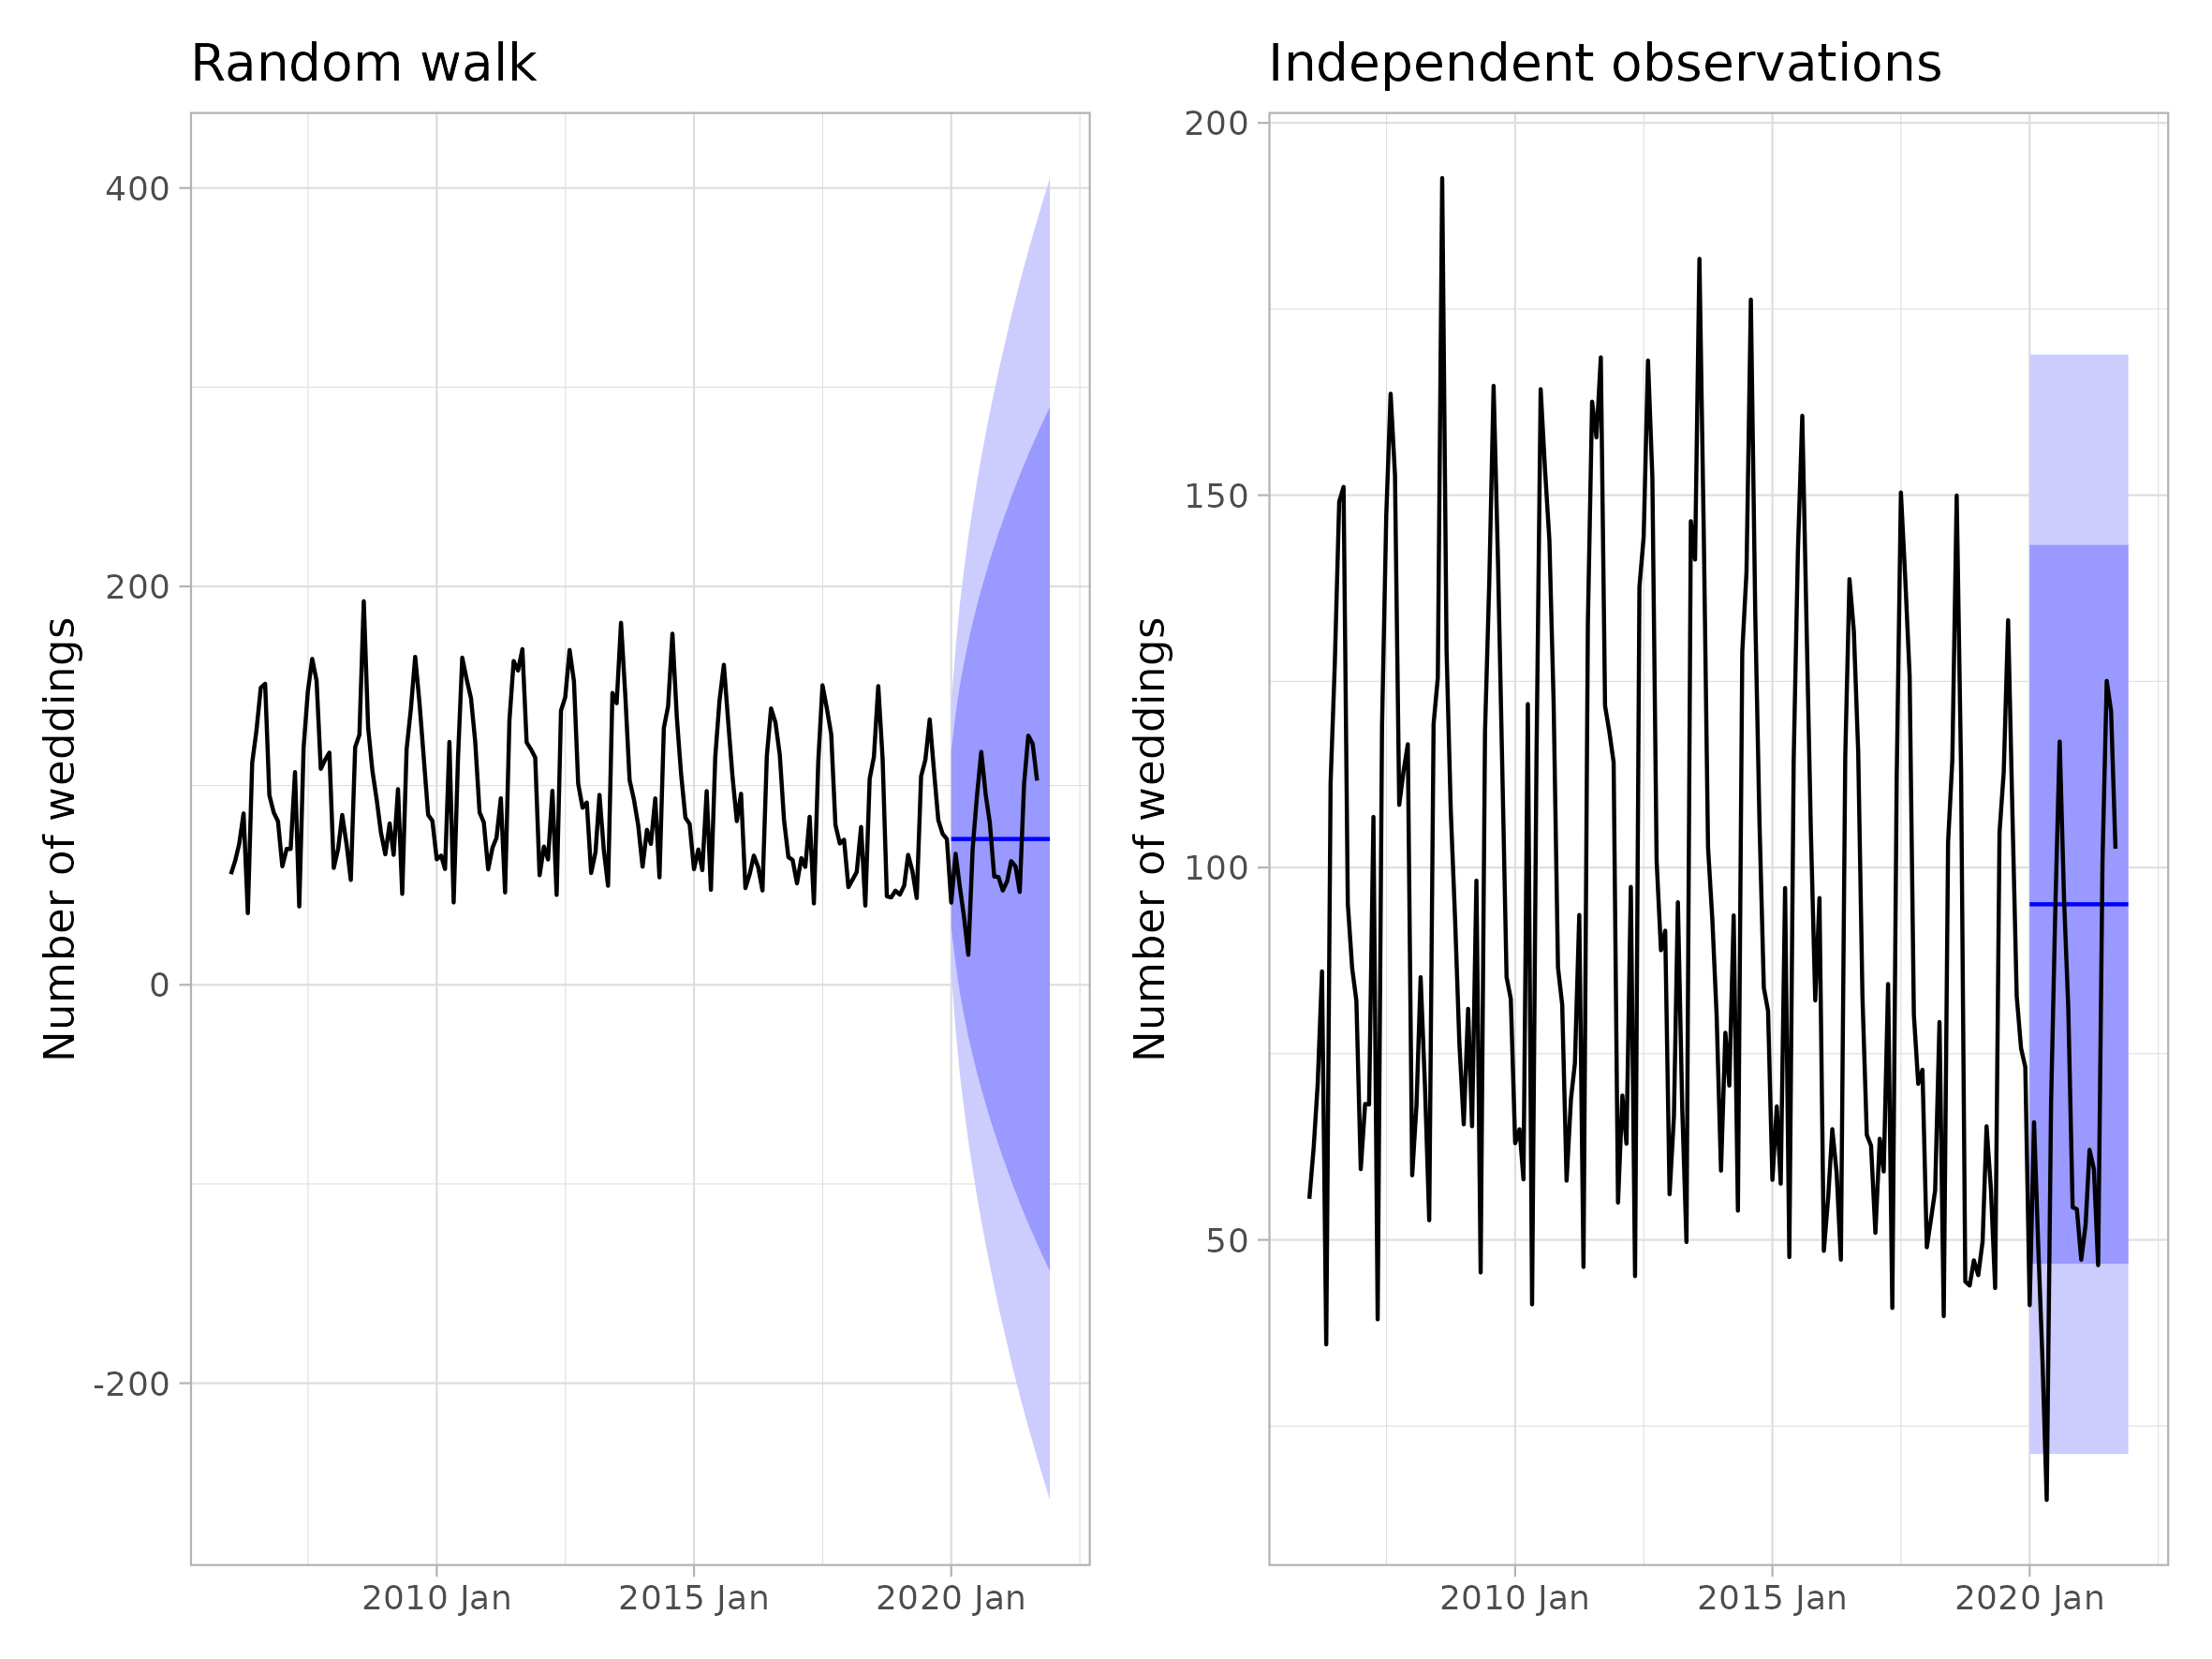
\includegraphics[width=\textwidth]{pictures/om_ts_01-157.png}
	
\end{frame}


\begin{frame}{Seasonal random walk}
	
	\begin{block}{Seasonal naive model}
		\[
		y_t = y_{t-12} + u_t,
		\]
		where $u_t$ is white noise, $u_t \sim \dN(0;\sigma^2)$, $y_1$, \ldots, $y_{11}$ are given
	\end{block}
	\pause
	Let's reformulate: $y_t - y_{t-12} = \Delta_{12} y_t = u_t$
	\pause
	
	\alert{Estimators:}
	\[
	\hat\sigma^2_{ML} = \frac{\sum(\Delta_{12} y_i - \overline {\Delta_{12} y})^2}{T - 12}
	\]
	\pause
	\alert{Interval forecast} for $h$ \alert{seasons} ahead:
	\[
	[y_{T} - 1.96 \hat \sigma \sqrt{h}; y_{T} + 1.96 \hat \sigma \sqrt{h}]
	\]
\end{frame}

\begin{frame}{Not bad already!}
	
	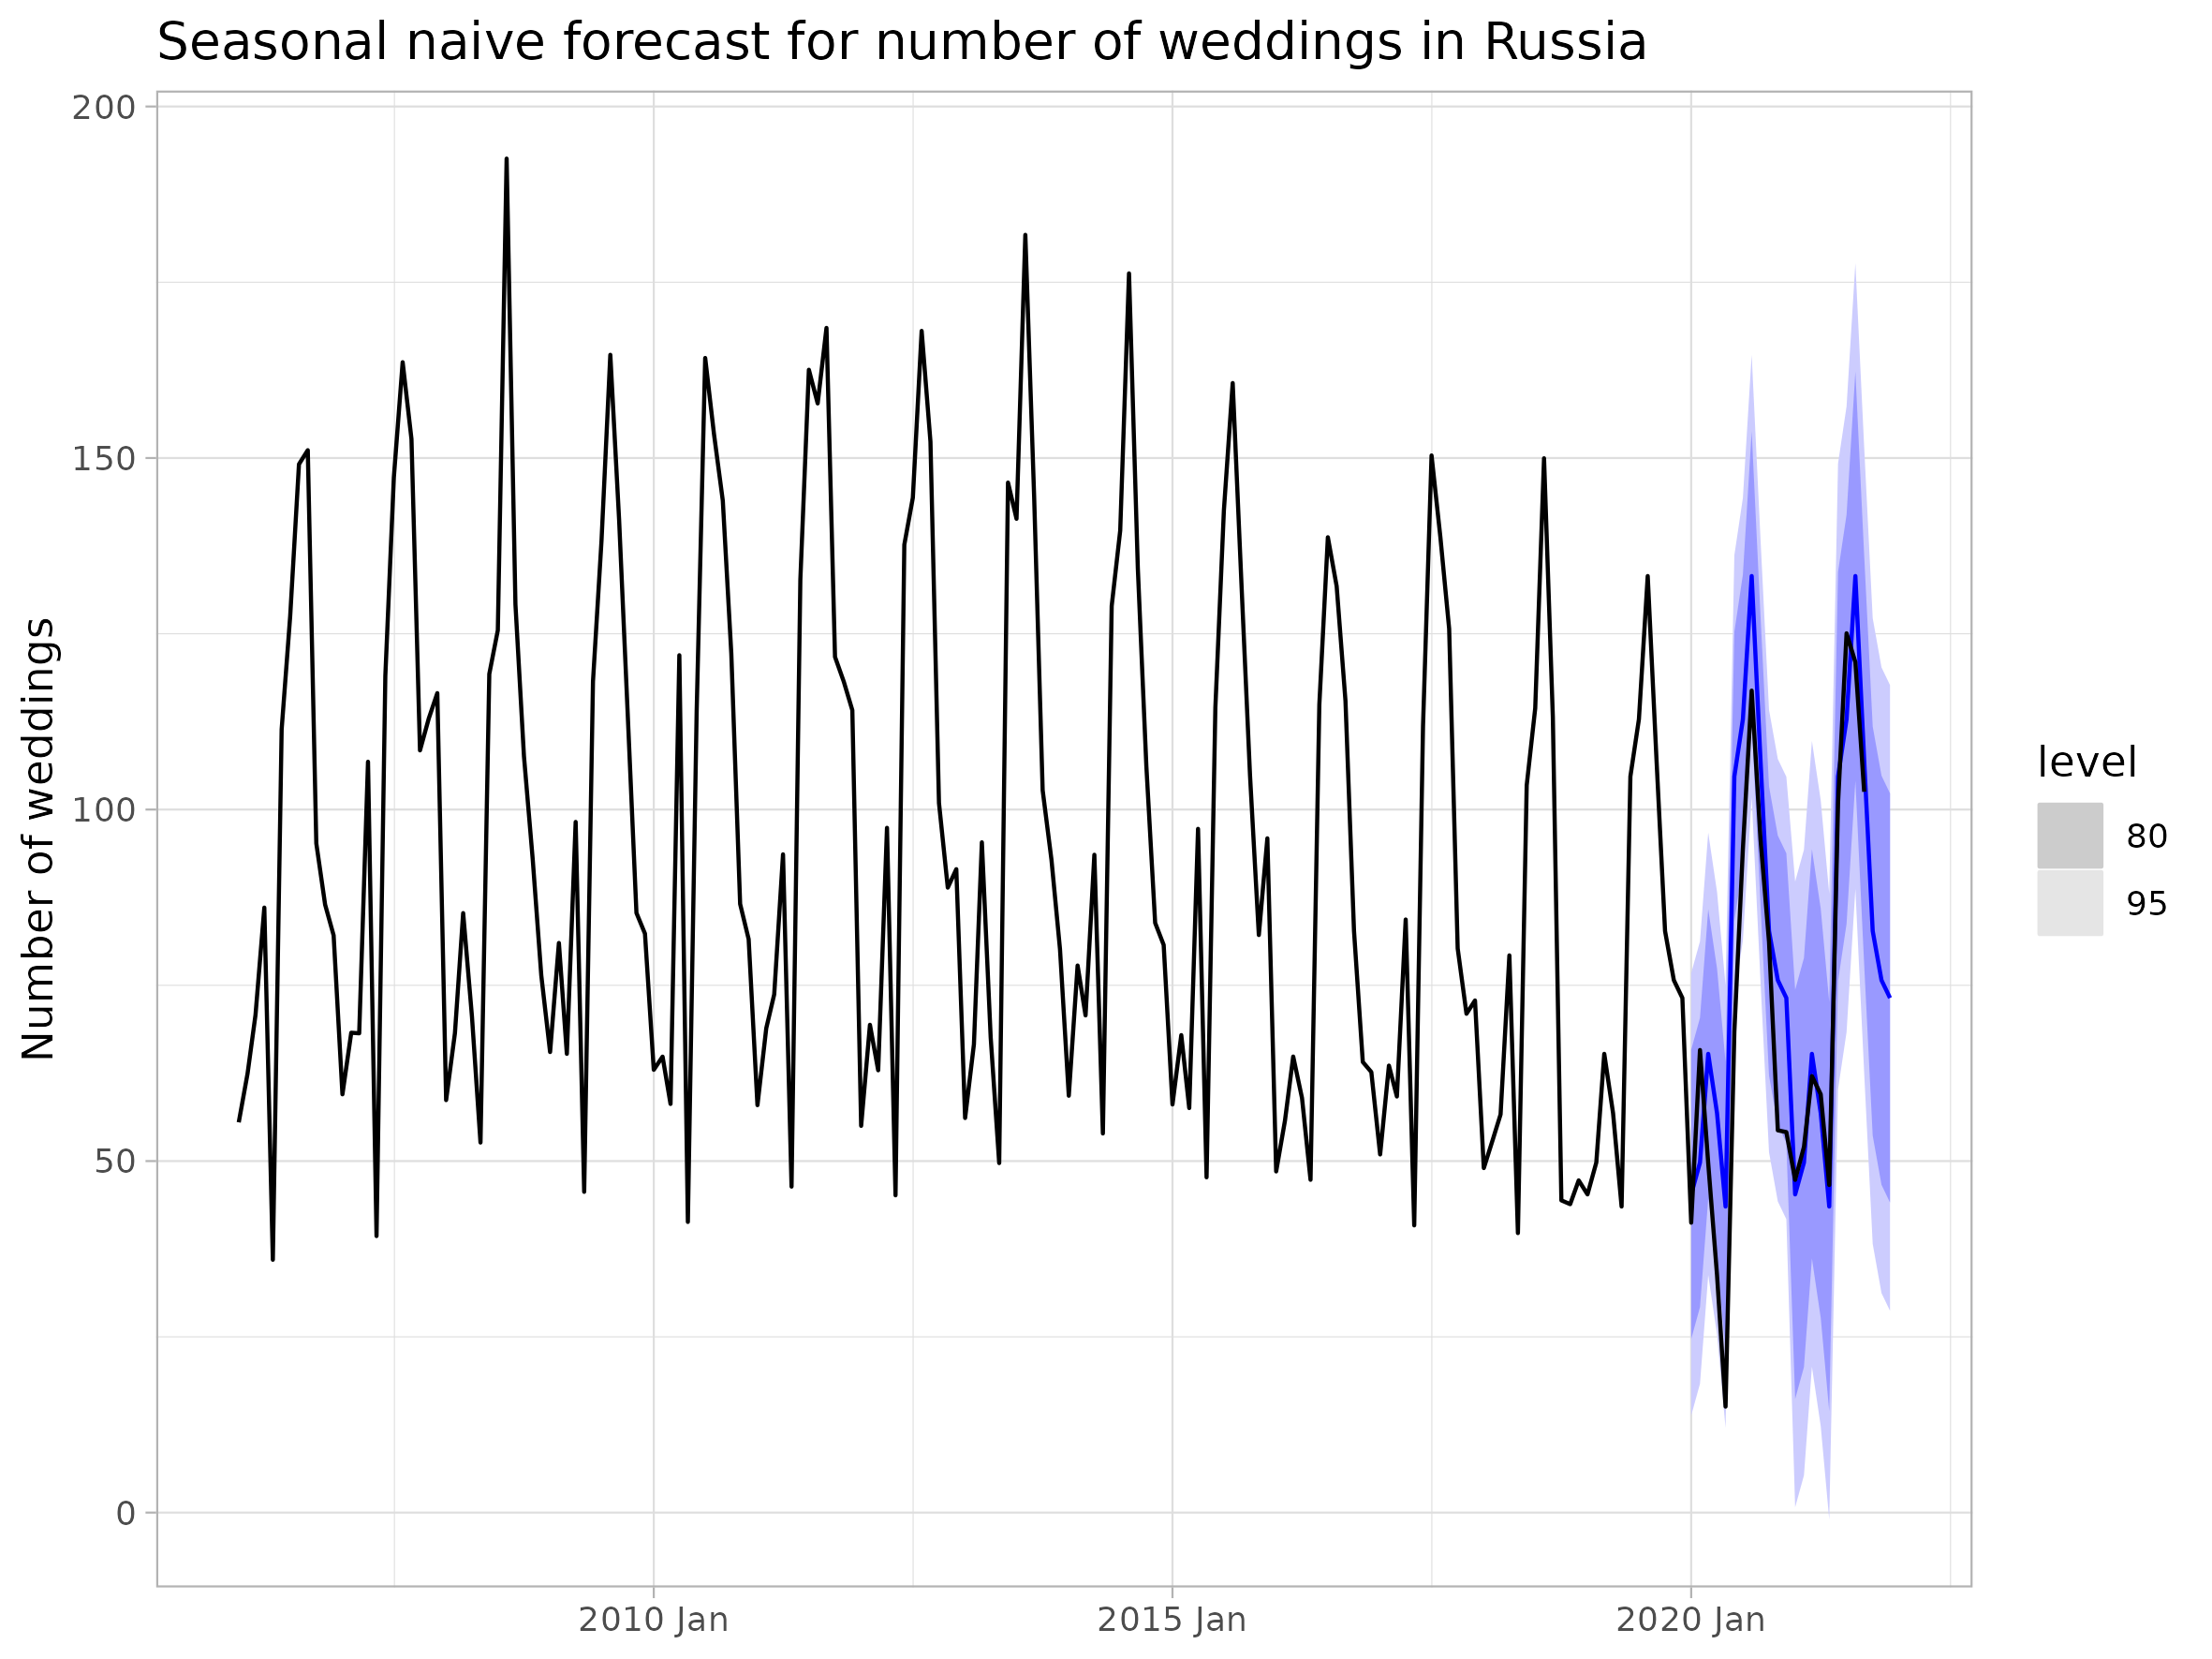
\includegraphics[width=\textwidth]{pictures/om_ts_01-162.png}
	
	
\end{frame}


\begin{frame}
	\frametitle{Why do we need naive models?}
	
	\begin{itemize}[<+->]
		\item \alert{Ideas} for complex model:
		
		the \alert{stationary series} models are similar to the independent observations model;
		
		\alert{non-stationary series} models are similar to a random walk
		
		\item \alert{Benchmark for comparison}:
		
		when evaluating a complex model, it is very important to have a base of comparison
		
		\item \alert{Averaging} with other models' forecasts:
		
		you can \alert{average forecasts} of a complex model and a naive seasonal one!
	\end{itemize}
	
	
\end{frame}

\begin{frame}{Naive Models: Summary}
	
	\begin{itemize}[<+->]
		\item White noise is what you don't want to simulate
		\item Independent observations and random walk
		\item Ideas, parts, and helpers for other models
		\item Base for comparison
	\end{itemize}
\end{frame}